% Metódy inžinierskej práce

\documentclass[10pt,twoside,slovak,a4paper]{article}

\usepackage[slovak]{babel}
%\usepackage[T1]{fontenc}
\usepackage[IL2]{fontenc} % lepšia sadzba písmena Ľ než v T1
\usepackage[utf8]{inputenc}
\usepackage{graphicx}
\usepackage{url} % príkaz \url na formátovanie URL
\usepackage{hyperref} % odkazy v texte budú aktívne (pri niektorých triedach dokumentov spôsobuje posun textu)

\usepackage{cite}
%\usepackage{times}

\pagestyle{headings}

\title{Nástroje CASE a ich využitie v reverznom inžinierstve\thanks{Semestrálny projekt v predmete Metódy inžinierskej práce, ak. rok 2021/22 vedenie: Vladimír Mlynarovič}} % meno a priezvisko vyučujúceho na cvičeniach

\author{Šimon Ukuš\\[2pt]
	{\small Slovenská technická univerzita v Bratislave}\\
	{\small Fakulta informatiky a informačných technológií}\\
	{\small \texttt{xukus@stuba.sk}}
	}

\date{\small 3. november 2021} 



\begin{document}

\maketitle

\begin{abstract}
Článok sa zaoberá problematikou softvérového inžinierstva, kontkrétne ako je možné proces vývoja softvéru automatizovať pomocou nástrojov CASE - Computer-Aided Software Engineering (Počítačom podporované softvérové inžinierstvo). V práci sa popisuje či už delenie týchto nástrojov,  tak aj sféry ich využitia.  Článok ďalej skúma softvérové inžinierstvo a použitie CASE nástrojov z inej perspektívy.  Na rozdiel od vnímania vývoja softvéru klasicky, teda smerom vpred (Forward Engineering) sa venuje tzv. spätnému inžinierstvu (Reverse Engineering). Tu je skúmaná kompletnosť a presnosť spätne navrhnutých UML diagramov generovaných nástrojmi CASE. Predmetom porovnania bolo celkom 8 nástrojov (z toho 6 open source a 2 komerčné). Tieto nástroje boli hodnotené na základe toho, aké typy vstupov podporujú, aké typy diagramov dokážu rekonštruovať a v akej kvalite.
 
\end{abstract}



\section{Úvod}
Pojem softvérové inžinierstvo môže byť chápaný ako uplatňovanie metód, postupov a nástrojov na riadenie a vývoj počítačových systémov \cite{1985} . Ide o komplexný postup, na ktorom sa zúčastňuje mnoho odborníkov z rôznych oblastí, ako napríklad projektový manažér, team líder, softvérový developer, tester, UI dizajnér a mnoho ďalších. Časť ich práce je možno automatizovať či uľahčiť využitím nástrojov CASE. Tieto nástroje sú špeciálne vyvinuté pre podporu vývoja softvéru, automatizujú proces vývoja. Cieľom ich implementácie je skrátenie času a nákladov pri vývoji softvéru a zvýšenie jeho kvality \cite{Osama:Adoption} .




Motivujte čitateľa a vysvetlite, o čom píšete. Úvod sa väčšinou nedelí na časti.

Uveďte explicitne štruktúru článku. Tu je nejaký príklad.
Základný problém, ktorý bol naznačený v úvode, je podrobnejšie vysvetlený v časti~\ref{nejaka}.
Dôležité súvislosti sú uvedené v častiach~\ref{dolezita} a~\ref{dolezitejsia}.
Záverečné poznámky prináša časť~\ref{zaver}.

toto je moj komentar :) Patrik
a toto je zas moj komentár :D L

\section{Nejaká časť} \label{nejaka}

Z obr.~\ref{f:rozhod} je všetko jasné. 

\begin{figure*}[tbh]
\centering
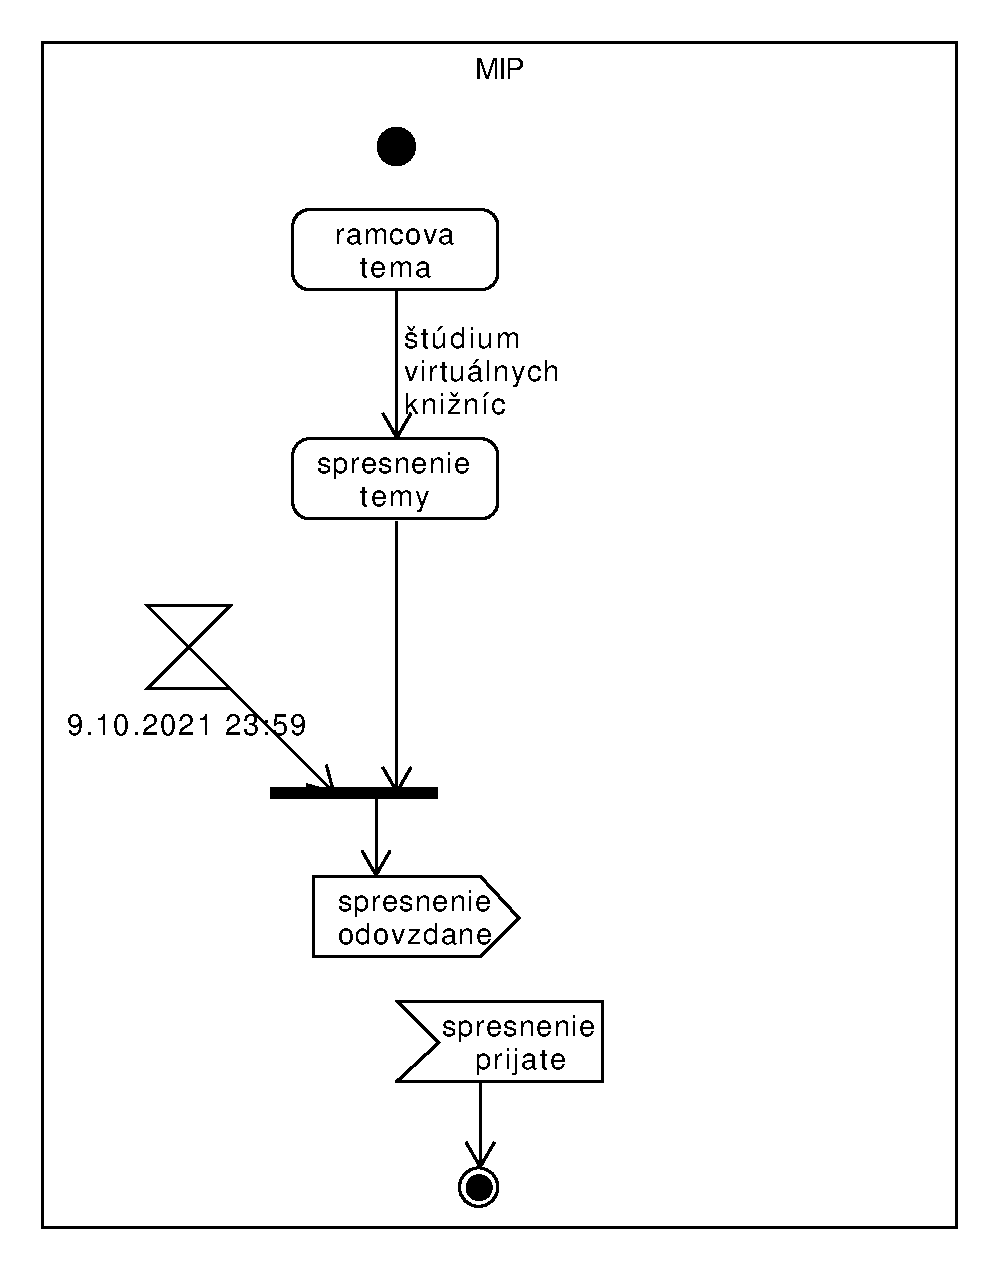
\includegraphics[scale=1.0]{diagram.pdf}
Aj text môže byť prezentovaný ako obrázok. Stane sa z neho označný plávajúci objekt. Po vytvorení diagramu zrušte znak \texttt{\%} pred príkazom \verb|\includegraphics| označte tento riadok ako komentár (tiež pomocou znaku \texttt{\%}).
\caption{Rozhodujúci argument.}
\label{f:rozhod}
\end{figure*}



\section{Iná časť} \label{ina}

Základným problémom je teda\ldots{} Najprv sa pozrieme na nejaké vysvetlenie (časť~\ref{ina:nejake}), a potom na ešte nejaké (časť~\ref{ina:nejake}).\footnote{Niekedy môžete potrebovať aj poznámku pod čiarou.}

Môže sa zdať, že problém vlastne nejestvuje\cite{Coplien:MPD}, ale bolo dokázané, že to tak nie je~\cite{Czarnecki:Staged, Czarnecki:Progress}. Napriek tomu, aj dnes na webe narazíme na všelijaké pochybné názory\cite{PLP-Framework}. Dôležité veci možno \emph{zdôrazniť kurzívou}.
\cite{Osman:RE} skúsim pridať citáciu \emph{toto bude zdôraznené}
Niekedy budem chcieť citovať toto \cite{Osama:Adoption}. OK?


\subsection{Nejaké vysvetlenie} \label{ina:nejake}

Niekedy treba uviesť zoznam:

\begin{itemize}
\item jedna vec
\item druhá vec
	\begin{itemize}
	\item x
	\item y
	\end{itemize}
\end{itemize}

Ten istý zoznam, len číslovaný:

\begin{enumerate}
\item jedna vec
\item druhá vec
	\begin{enumerate}
	\item x
	\item y
	\end{enumerate}
\end{enumerate}


\subsection{Ešte nejaké vysvetlenie} \label{ina:este}

\paragraph{Veľmi dôležitá poznámka.}
Niekedy je potrebné nadpisom označiť odsek. Text pokračuje hneď za nadpisom.



\section{Dôležitá časť} \label{dolezita}




\section{Ešte dôležitejšia časť} \label{dolezitejsia}



\section{Záver} \label{zaver} % prípadne iný variant názvu



%\acknowledgement{Ak niekomu chcete poďakovať\ldots}


% týmto sa generuje zoznam literatúry z obsahu súboru literatura.bib podľa toho, na čo sa v článku odkazujete
\bibliography{literatura}
\bibliographystyle{abbrv} % prípadne alpha, abbrv alebo hociktorý iný
\end{document}
